% This is "sig-alternate.tex" V2.0 May 2012 This file should be compiled
% with V2.5 of "sig-alternate.cls" May 2012
% 
\documentclass{sig-alternate-10pt} \usepackage{enumerate}
\usepackage{hyperref} 
\usepackage{url}
\usepackage{tikz}

\newcommand*\mycirc[1]{%
  \begin{tikzpicture}
    \node[draw,circle,inner sep=1pt] {#1};
  \end{tikzpicture}}
  
\begin{document}

\title{Federation over SSH}
\author{
Ravishankar Muniraju
}

\maketitle

\section{Introduction}


\begin{figure*}
  \begin{center}
    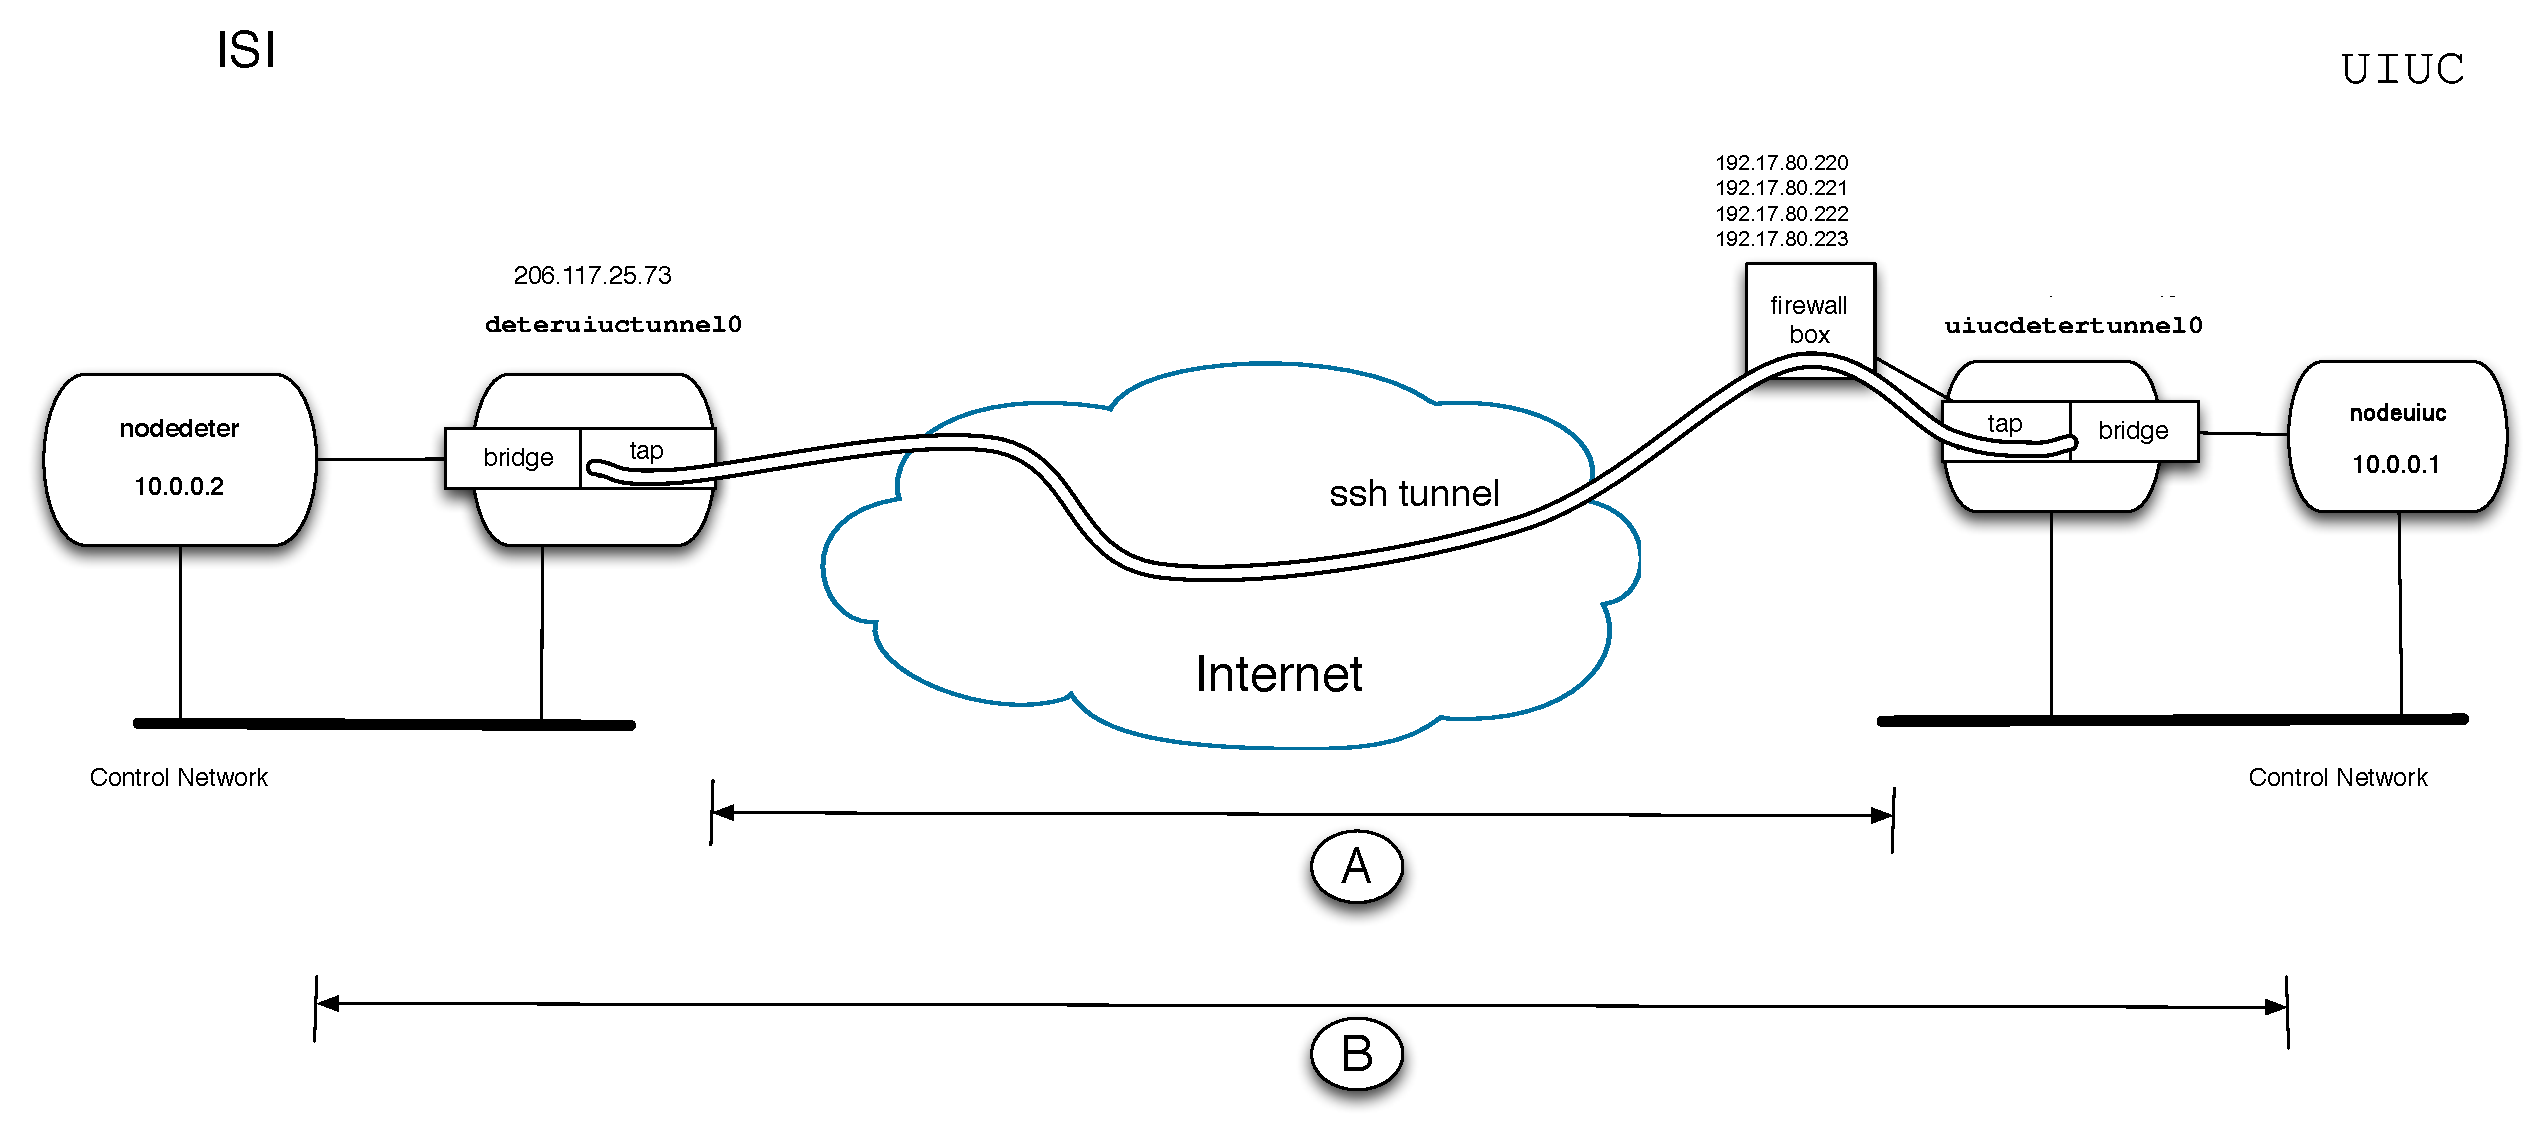
\includegraphics[width=6in]{figures/deter-uiuc-feddmap.pdf} 
    \caption{A conceptual representation of the federation link between ISI and UIUC}
    \label{fig:isi-uiuc}
  \end{center} 
\end{figure*}

Federation is a well established technology is DETER and is  widely used 
 for experimentation. 
We recently started to explore using federation in the DEFT 
 consortium to model  energy cyber physical systems
 distributed across three federated testbeds at PNNL, UIUC and ISI. 
This note presents an empirical characterization of a DETER federation link 
between the ISI DETER testbed located at Marina del Rey, CA and the UIUC
DETER testbed located at  Illinois. 

The empirical characterization of the federated link 
 can be used to inform the energy cyber 
physical models developed as part of the DEFT consortium. 
The DEFT consortium is exploring dependent, time synchronized 
 CPS models that will span the across the three testbeds. 
Such models are delay sensitive. 
 Hence it is important to
quantify the delay properties of the underlining cyber substrate so that the
models can correctly designed for this environment.

As seen in Figure~\ref{fig:isi-uiuc}, 
 the DETER federation framework sets up 
an ssh tunnel between the two testbeds.
All traffic between the testbed nodes, nodedeter and nodeuiuc, 
 is subsequently transfered over the tunnel by directly bridging the 
 the end node to the ssh tunnel using a federation \emph{tap}. 

In this note, based on the ISI--UIUC federation as an example, 
 we show that DETER federation link reports a latency measurement average
  which is ---(to be decided after a required measurement is obtained) times higher than the underlying internet link.
The impact of this latency is also seen in the applications
 running on the end nodes. 
 This increased latency makes it 
  challenging to 
  design
 delay sensitive and time-synchronized 
  applications for energy cyber physical systems. 

%We evaluate both the connectivity and capacity properties of the
%interconnect. 
We discuss our empirical evaluation 
 methodology in Section~\ref{sec:approach}. In section ~\ref{sec:perfomance metrics} we discuss the performance metrics 
 used to characterize the links. We
perform measurement analysis and observation in Section~\ref{sec:Observation}.
In Section~\ref{sec:pathforward}, we discuss possible directions that we
can follow to get more insight into the properties of the federation substrate and
improve its performance.

\section{Methodology} 

  The Methodology used here is very similar to  ~\cite{wang06}.
  We are using a active UDP probing mechanism to characterize the federation link.
Probing mechanism involves sending a burst of UDP packets of size 46bytes with a certain {\it inter burst time}. Upon arrival of the each UDP packet, destination node records the timestamp and sequence number
of the UDP packet received. 

\label{sec:approach}

\subsection{Connectivity}

\begin{figure} 
  \begin{center}
    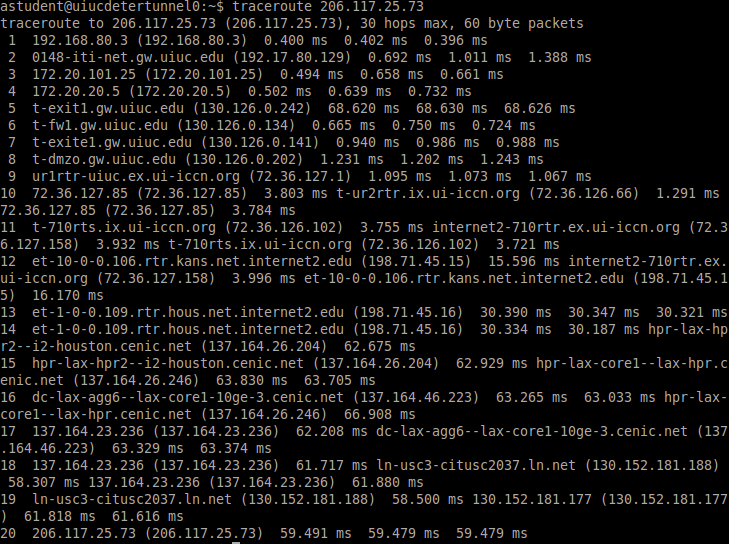
\includegraphics[width=3in]{traceroute_uiuctunnel2detertunnel.png}
    \caption{The output from $traceroute$ between UIUC tunnel and ISI tunnel }
    \label{fig:uiucisitraceroute} 
    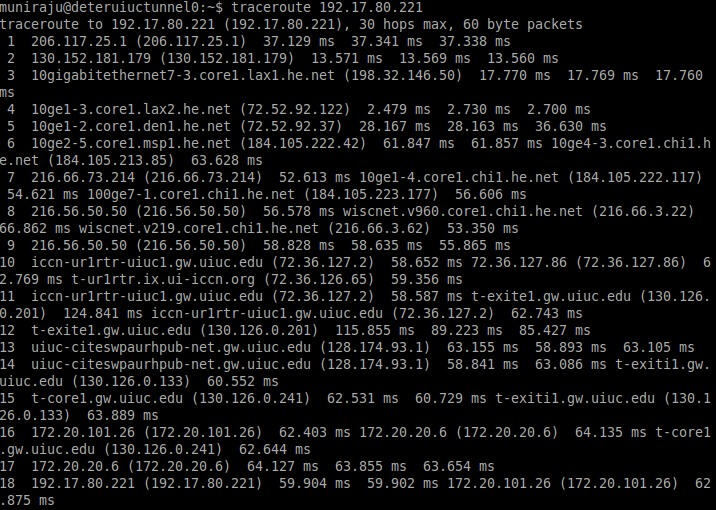
\includegraphics[width=3in]{traceroute_detertunnel2uiuctunnel.png}
    \caption{The output from $traceroute$ between ISI tunnel and UIUC tunnel }
    \label{fig:isiuiuctraceroute} 
  \end{center} 
\end{figure}


We use traceroute to find the network path from UIUC to ISI and viceversa. 
The traceroute from UIUC to ISI, (shown in
 Figure~\ref{fig:uiucisitraceroute} ) indicates the path from UIUC to ISI first 
 traverses a few servers at University of Urbana champaign, then traverses
 throught Internet2 server at Ann Arbor, Michigan, Cenic network at Cypress, CA and finally traverses
 Los Nettos (\url{http://www.ln.net/}), a small regional ISP, that
provides connectivity to USC/ISI.
\\Figure~\ref{fig:isiuiuctraceroute} indicates the path from ISI to UIUC. first 
 traverses Los nettos, then traverses the following ISPs - Telehouse International Corp. Of America in Los angeles, Hurricane Electric Inc in Los angeles followed by the same ISP at colorado and chicago, Wiscnet in winsconsin, finally traverses few servers at  University of Urbana champaign to reach the final destination.

%The reverse path, from PNNL to ISI is completely dark. Traceroute does not provide any
% information about that path.



\section{Perfomance metrics} 
\label{sec:perfomance metrics}

In our study we have used the following metrics to characterize the federation link.

\subsection{Packet loss} 
\label{sec:Packet loss}

We identify the loss by observing the gaps in the sequence numbers of received UDP probe packets.
We use a metrics called {\it bursty loss size}, which is defined as the maximum number of consecutive
packets lost between two in-order packets. 

%We empirically estimate the properties of the interconnect between
%ISI-PNNL using 
%ping and 
%nuttcp (\url{http://www.nuttcp.net} 
%measurements.
\subsection{Packet delay} 
\label{sec:Packet delay}

Ideally we need to measure the one way delay, but this is limited by the clock synchronisation at deter testbed at ISI and
deter testbed in UIUC. Hence we measure the round trip time using the UDP packets used for probing. The RTT calculation here is similar to what was done in ~\cite{SRM}
Each UDP probe packet sent is timestamped and sequenced. Let us assume a packet P1 sent at time t1. P1 reaches nodeuiuc at t2. nodeuiuc
will now consrtuct UDP packet P2 which includes two time stamp values t1 and t2-t3(time spend in nodeuiuc system) where t3 is the time at which the nodeuiuc
sends P2. Let P2 reach nodedeter at t4. Once P2 receives nodedeter, it estimates the round trip time between nodedeter and node uiuc using the following formula {\textbf {RTT = t4-t1-(t3-t2)}}.
 We estimate the rtt for one in every ten packets the nodeuiuc receives.

\subsection{Jitter}
\label{sec:Jitter}
Initially we calculate the inter-arrival time of the packets received using which we proceed to 
calculate the jitter. Jitter is calculated for both in-order and out-of-order packets.

\subsubsection{In order packets}
\label{sec:Jitterinorder}


 Two in order packets arriving one after the other at receiving node
 may belong to same or different bursts. If the packets belong to same burst burst then the inter-arrrival time is equal to the jitter.
 Where as if the packets belong to different bursts then the jitter is calculate as shown:
\\*
{\textbf {jitter = (inter-arrival time) - (burst difference * {\it {burst inter time})}}.


\subsubsection{Out of order packets}
\label{sec:Jitter out of order}


 If an out of order packet arrives at receiving node, first we find the UDP packet that was received with highest, but lower than the out of order sequence number received. Find the inter-arrival time between these two packets and then calculate the jitter using the equation used to calculate jitter for in order packets.

\subsection{Bandwidth and Flow completion time} 
\label{sec:bandwidthflowtime}
NutTCP is a network measurement tool
 that reports the available bandwidth between 
  two locations. 
We use NutTCP to measure available bandwidth between testbeds at ISI and UIUC along path \mycirc{B} and \mycirc{A} . 
 The application continuously transfers a 100MB block of data 
  from ISI to UIUC using tcp every 10 seconds. 
For each transfer, NutTCP reports the available bandwidth and flow completion time. 







\section{Observations and Analysis}
\label{sec:Observation}
\subsection{Characterization of path along \bf{A} and \bf{B}}
In this section we are characterizing the link along path \mycirc{A} and \mycirc{B} and comparing 
their performance. we obtain packet delay, jitter and packet loss using the UDP probing mechanism which sends
a UDP packet every 5 msec. The bandwidth and flow completion time is obtained using nuttcp as described in Section ~\ref{sec:bandwidthflowtime}.

\subsubsection{Bandwidth and flow time}
\label{sec:BandFT}
We measure the bandwidth and the flow completion time as described in Section ~\ref{sec:bandwidthflowtime}.
Figures ~\ref{fig:nodebwft} and  ~\ref{fig:tunnelbwft}  reports the bandwidth in Mbps along left y axis, flow completion time in seconds along the right y axis and epoch time in hours along x 
axis for measurements along path \mycirc{B} and \mycirc{A} respectively.

Figures ~\ref{fig:tunnelbw} and ~\ref{fig:nodebw}  shows the cdf plot of bandwidth in Mbps along path \mycirc{A} and \mycirc{B} respectively.
Figures ~\ref{fig:tunnelft} and ~\ref{fig:nodeft}  shows the cdf plot of flow completion time in seconds along path \mycirc{A} and \mycirc{B} respectively.
Statistics for both the paths are as shown in the table ~\ref{table:bwft}.
\begin{figure} 
  \begin{center}

    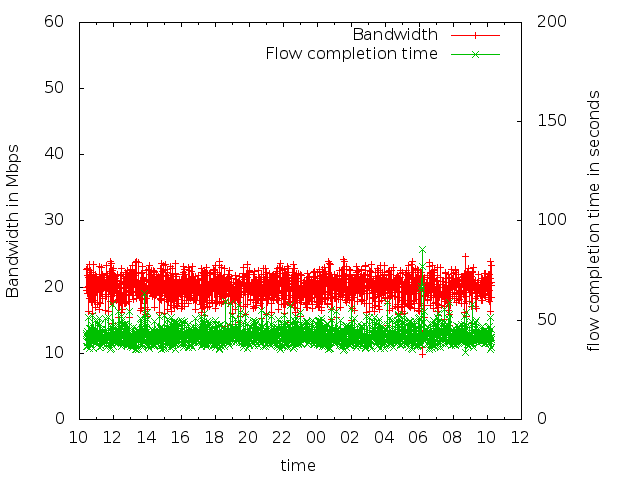
\includegraphics[width=2in]{figures/N2N/bandwidth_plot.png}
    \caption{bandwidth in Mbps and flow completion time in seconds along path \bf{B} }
    \label{fig:nodebwft} 

    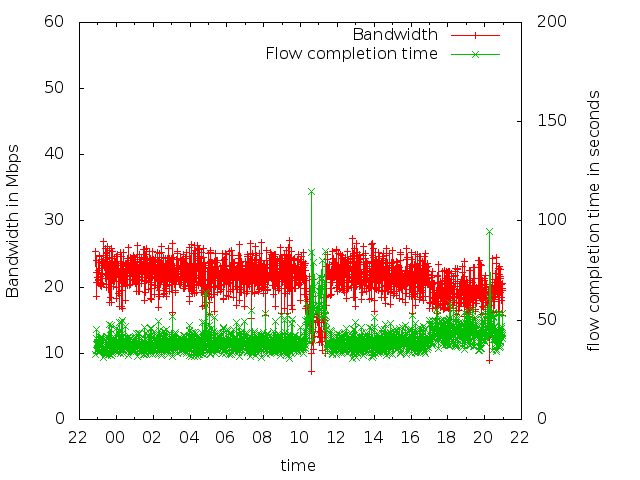
\includegraphics[width=2in]{figures/T2T/bandwidth_plot.png}
    \caption{bandwidth in Mbps and flow completion time in seconds along path \bf{A}}
    \label{fig:tunnelbwft} 
    
  \end{center} 
\end{figure}

\begin{figure} 
  \begin{center}

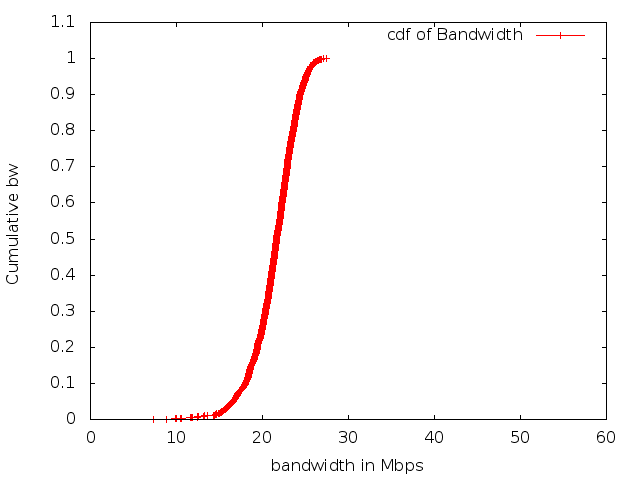
\includegraphics[width=2in]{figures/T2T/bandwidth_cdfplot.png}
    \caption{Cdf of bandwidth in Mbps along path \bf{A} }
    \label{fig:tunnelbw} 
    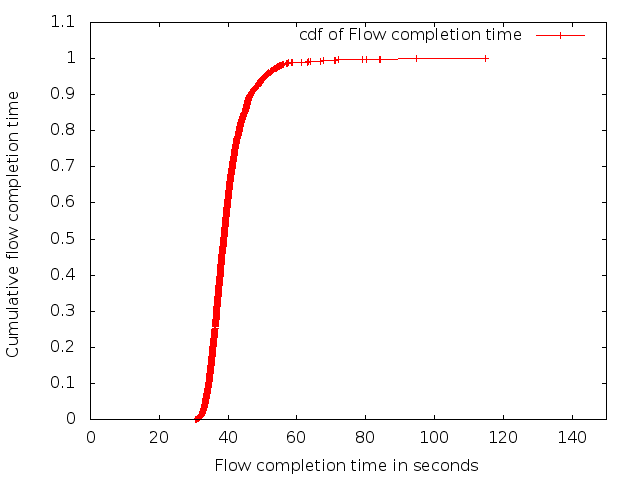
\includegraphics[width=2in]{figures/T2T/flowtime_cdfplot.png}
    \caption{Cdf of flow completion time in seconds along path \bf{A} }
    \label{fig:tunnelft}


\end{center} 
\end{figure}

\begin{figure} 
  \begin{center}
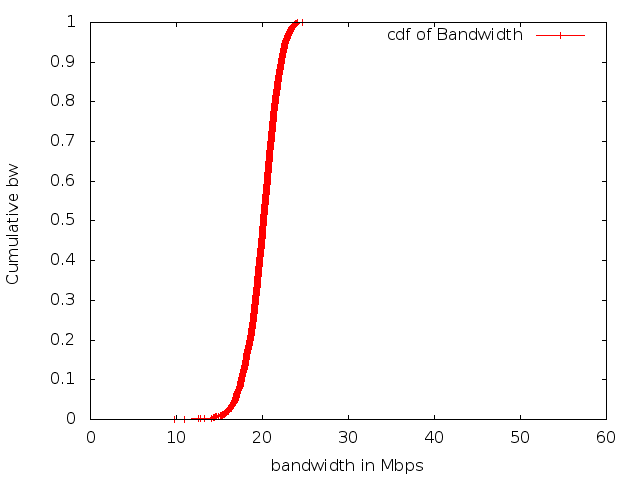
\includegraphics[width=2in]{figures/N2N/bandwidth_cdfplot.png}
    \caption{Cdf of bandwidth in Mbps along path \bf{B} }
    \label{fig:nodebw} 
    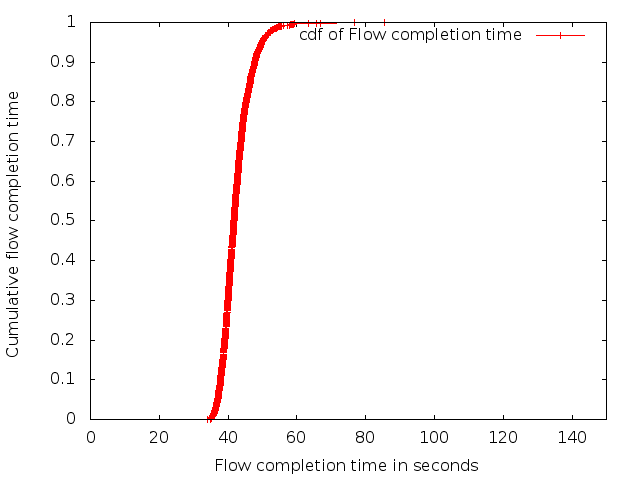
\includegraphics[width=2in]{figures/N2N/flowtime_cdfplot.png}
    \caption{Cdf of flow completion time in seconds along path \bf{B} }
    \label{fig:nodeft} 
  \end{center} 
\end{figure}


\begin{table}[ht]
\small
\caption{Bandwidth and flow time measurements along path \bf{A} and \bf{B}}

% title of Table
\centering
% used for centering table
\begin{tabular}{ |l | l | l |}
% centered columns (4 columns)
\hline
\hline %inserts double horizontal lines
 & \mycirc{A} & \mycirc{B}\\[0.5ex]
% inserts table
%heading
\hline
% inserts single horizontal line
Mean bandwidth in Mbps  & 21.37 &  19.958 \\
% inserting body of the table
Maximum bandwidth in Mbps & 27.11 & 24.10 \\
90\% Bandwidth in Mbps & <22 & <20 \\
Mean Flow completion time in seconds & 39.97 & 42.35 \\
% inserting body of the table
Maximum Flow completion time in seconds & 114.97 & 85.49 \\
90\% Flow completion time in seconds & <=40 & 42 \\[1ex]
% [1ex] adds vertical space
\hline
%inserts single line
\end{tabular}
\label{table:bwft}
% is used to refer this table in the text
\end{table}

{ \it Implications: We can observe that the bandwidth is higher in along \mycirc{A} and lower along \mycirc{B}. The reason being the packets along the path}
{\it \mycirc{B} flows through the ssh tunnel hence incurring addition latency where as the packets along the path \mycirc{A} doesnt. This results in increase in} 
{\it flow completion time along \mycirc{B}.} 



%Bandwidth and flow time comparison between nodde and tunnel end %


%comparing within path A
\subsubsection{RTT, Jitter and Packet loss}
\label{sec:RJPL}
{\it TODO : Need to take readings of N=1 and  inter burst time = 5msec along node2node to complete this section }



\subsection{Characterization of path along \bf{A} }
In this section we are characterizing the link along path \mycirc{A} and comparing 
their performance. we obtain packet delay, jitter and packet loss using the UDP probing mechanism.
Jitter and packet delay are calculated as described in section ~\ref{sec:Jitter} and ~\ref{sec:Packet delay} respectively.

\subsubsection{Packet delay and Jitter}
To measure and analyze RTT and jitter along the path \mycirc{A} we use UDP probing mechanism by sending packets with the following inter packet times:
\\ Case 1 : 10msec
\\ Case 2 : 5msec
\\ Case 3 : 15msec : To be done


Figures ~\ref{fig:tunnelrtt10} and  ~\ref{fig:tunnelrtt5}  reports the cdf of packet delay in microseconds for Case 1 and 2 respectively.
Figures ~\ref{fig:tunneljitter10} and  ~\ref{fig:tunneljitter5}  reports the cdf of jitter in microseconds for Case 1 and 2 respectively.

Statistics for packet delay and jitter for cases 1, 2 and 3 are as shown in the table ~\ref{table:tunnelrttjitter}.

\begin{table}[ht]
\small
\caption{Packet delay and jitter measurements along path A for cases 1, 2 and 3}

% title of Table
\centering
% used for centering table
\begin{tabular}{|l|l|l|l|}
% centered columns (4 columns)
\hline
\hline %inserts double horizontal lines
 & case1 & case2 & case3 \\[0.5ex]
% inserts table
%heading
\hline
% inserts single horizontal line
Mean Packet delay in usec  &62479  &62780   & \\
% inserting body of the table
Maximum Packet delay in usec & 340654 &2271468  &\\
%90\% Packet delay in usec & <64000 & <65000 &\\
Mean Jitter in usec & 332.33 &343  &\\
% inserting body of the table
Maximum Jitter in usec & 280317 & 1805360 & \\
%95\% Jitter in usec & <300  & <300 &\\[1ex]
% [1ex] adds vertical space
\hline
%inserts single line
\end{tabular}
\label{table:tunnelrttjitter}
% is used to refer this table in the text
\end{table}




\begin{figure} 
  \begin{center}

    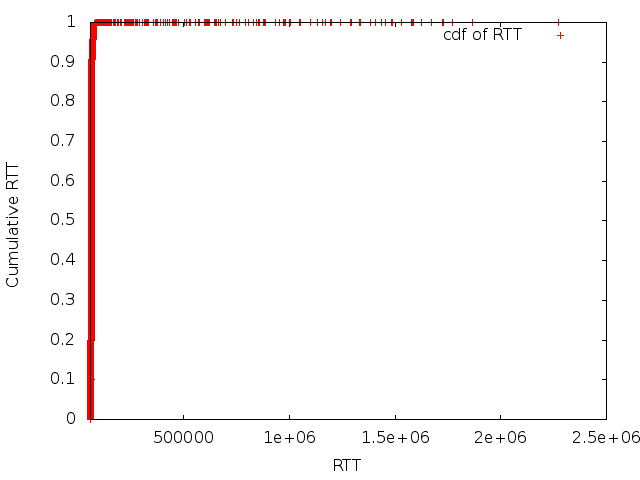
\includegraphics[width=2in]{figures/T2T/rtt_cdfplot_1_5ms.png}
    \caption{RTT in micro seconds along path \bf{A} for inter packet time equal to 5msec }
    \label{fig:tunnelrtt5} 

    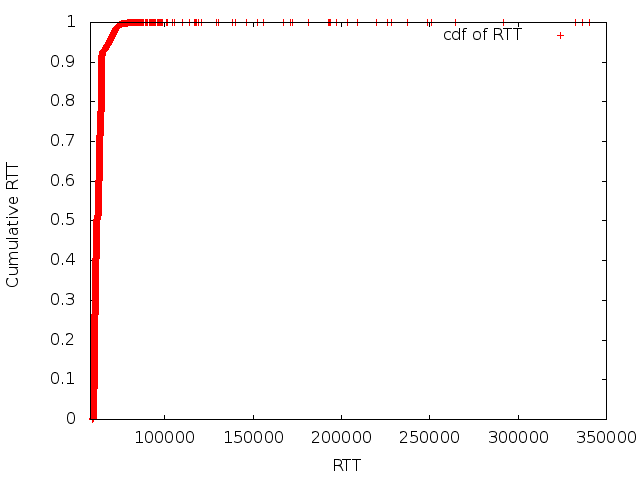
\includegraphics[width=2in]{figures/T2T/rtt_cdfplot_1_10ms.png}
    \caption{RTT in micro seconds along path \bf{A} for inter packet time equal to 10msec}
    \label{fig:tunnelrtt10} 
    
  \end{center} 
\end{figure}

\begin{figure} 
  \begin{center}

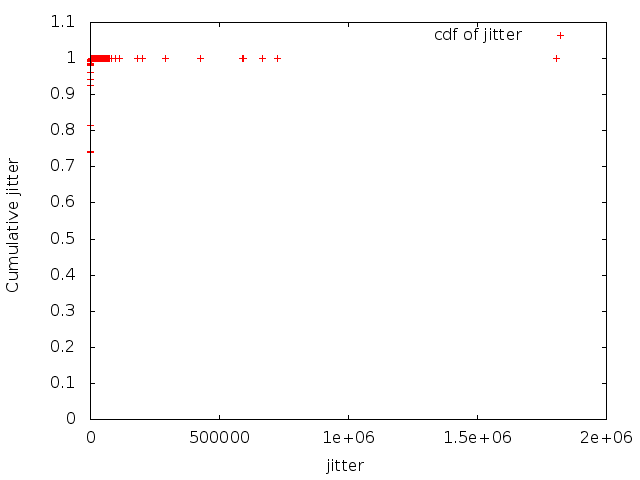
\includegraphics[width=2in]{figures/T2T/jitter_cdfplot_1_5ms.png}
    \caption{Cdf of Jitter in micro seconds along path \bf{A} for inter packet time equal to 5msec}
    \label{fig:tunneljitter5} 
    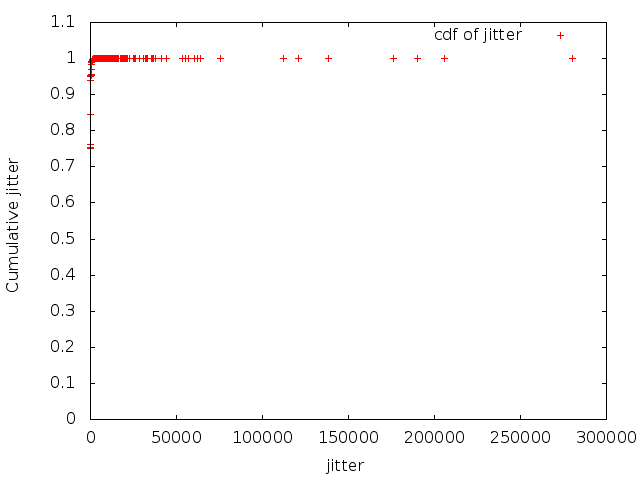
\includegraphics[width=2in]{figures/T2T/jitter_cdfplot_1_10ms.png}
    \caption{Cdf of Jitter in micro seconds along path \bf{A} for inter packet time equal to 10msec }
    \label{fig:tunneljitter10}


    
  \end{center} 
\end{figure}


{ \it Implications: Control signals sent along the path \mycirc{A} at 5msec suffer very high packet delays and jitter as shown in the table ~\ref{table:tunnelrttjitter}} 
{\it and in the figures ~\ref{fig:tunnelrtt5} and ~\ref{fig:tunneljitter5}. In Case1 we transmit packets at half the rate of Case2. Decrease in the rate by half results in atmost 6 times decrease in the RTT and jitter.} 



\subsubsection{Packet loss}
To measure and analyze packet losses along the path \mycirc{A} we use UDP probing mechanism by sending packets with inter-burst time of 50msec and with the following burst lengths:
\\ Case 1 : burst length = 2
\\ Case 2 : burst length = 5
\\ Case 3 : burst length = 10






%Figures ~\ref{fig:tunnelloss5} and  ~\ref{fig:tunnelloss10}  reports the cdf of {\it burst loss size} in number of packets for burst lenght equal to 5 and 10 %respectively.


Statistics of {\it burst loss size} for Case 1 and Case 2 are as shown in the table ~\ref{table:tunnelloss}.

\begin{table}[ht]
\small
\caption{{\it burst loss size} measurements along path A for burst length 5 and 10}

% title of Table
\centering
% used for centering table
\begin{tabular}{|l|l|l|l|}
% centered columns (4 columns)
\hline
\hline %inserts double horizontal lines
 & case1 & case2 &case3\\[0.5ex]
% inserts table
%heading
\hline
% inserts single horizontal line
Percentage of lost packets  &0.08 &0.16  &1.8  \\
% inserting body of the table
%Mean {\it burst loss size} in packets  & 340654 &2271468 \\
%90\% Packet delay in usec & <64000 & <65000 &\\
%Number of bursts & 332.33 &343 \\
% inserting body of the table
%95\% Jitter in usec & <300  & <300 &\\[1ex]
% [1ex] adds vertical space
\hline
%inserts single line
\end{tabular}
\label{table:tunnelloss}
% is used to refer this table in the text
\end{table}





{ \it Implications: We observe an increase in the percentage of lost packets as we increase the burst size as shown in the table ~\ref{table:tunnelloss} } 




\section{Observation and Path Forward}
\label{sec:pathforward}


/*To be filled later after discussing with the Professor*/

\bibliographystyle{abbrv} 
\bibliography{mybibfile}

 

\end{document}
